\section {Implementação de um servidor NTP de \textit{stratum} 1}

\subsection {Introdução}

O protocolo NTP implementa diversas soluções que permitem a sincronização dos
relógios dos computadores pertencentes a uma determinada rede. O protocolo
utiliza diversas métricas, descritas nas próximas seções, a fim de determinar
quais são as fontes mais seguras e consistentes para obter a melhor
sincronização e uma maior precisão. Somadas a essas estatísticas, o NTP faz uso
de algoritmos de seleção, \textit{cluster} e combinação que garantem, por sua
vez, a determinação dos servidores mais confiáveis a partir de um número finito
de amostras provindas de tais fontes. 

\vspace{12pt}

A troca de mensagens é feita através de pacotes UDP, sendo que o protocolo
suporta tanto o IPv4 quanto o IPv6. Apesar do fato de que o protocolo UDP não
oferece garantias de entrega e correção de eventuais erros ou duplicatas, o
NTPv4 implementa mecanismos, tais como o \textit{On-Wire protocol}, capazes de
verificar a consistência dos dados contidos nos pacotes recebidos e, assim,
agir corretamente em casos de perdas ou pacotes repetidos. 

\vspace{12pt}

Neste relatório, serão discutidas as características da versão 4 do NTP,
especificadas no RFC5905 \cite{ntpv4rtp}, e sua aplicação no contexto do sistema
do controle do acelerador \textit{Sirius}. Esta versão aprimora alguns aspectos
da versão 3 (NTPv3) e adiciona algumas outras funcionalidades, como, por exemplo, a
descoberta dinâmica de servidores (\textit{automatic server discovery}),
sincronização rápida na inicialização da rede ou depois de falhas (\textit{burst
mode}) e uso da criptografia \textit{Public-key}.

\subsection {Características do Protocolo}

O primeiro aspecto importante do protocolo NTPv4 é a organização dos
nós de uma rede. O NTP provê 3 tipos diferentes de variantes 
e 6 modos de associação, que identificam a função de cada nó que
compõe um comunicação. As variantes NTP são, portanto:

\begin {enumerate}[i.]
  
  \item \textit{server/client}: um cliente envia pacotes a um servidor
  requisitando sincronização, que responde utilizando o endereço contido nos
  respectivos pacotes. Nesta variante, servidores fornecem sincronização aos
  clientes, mas não aceitam sincronizações vindas deles. As associações
  entre os nós nesta variante são persistentes, ou seja, são criadas na
  inicialização do serviço e nunca são destruídas.
  
  \item \textit{symmetric}: neste tipo de variante, um nó se comporta tanto como
  servidor como cliente, isto é, ele recebe e envia informações de sincronização
  ao outro nó. Associações deste tipo podem ser persistentes, conforme explicado
  no item anterior, ou temporárias, isto é, podem ser criadas a partir do
  recebimento de um pacote e eliminadas após um certo intervalo ou ocorrência
  de erro. No primeiro caso, adota-se uma associação \textit{ativa}, enquanto
  que na segunda, adota-se uma \textit{passiva}.
      
  \item \textit{broadcast}: nesta variante, um servidor \textit{broadcast}
  persistente envia pacotes que podem ser recebidos por diversos clientes.
  Quando um cliente recebe um pacote deste tipo, uma associação temporária do
  tipo \textit{broadcast client} é criada e o cliente recebe sincronização até o
  fim de um intervalo ou ocorrência de um erro.
  
\end{enumerate}

O protocolo oferece ainda uma funcionalidade que permite aos clientes
descobrirem servidores disponíveis na rede para sincronização. Tal mecanismo é
chamado de \textit{Dynamic Server Discovery}, que provê dois tipos especiais de
associação: \textit{manycast server} e \textit{manycast client}. Um cliente
\textit{manycast} persistente envia pacotes para endereços de \textit{broadcast}
ou \textit{multicast} e, caso um \textit{manycast server} receba tais pacotes,
ele envia uma resposta a determinado cliente, que, por sua vez, mobiliza uma
associação temporária com o respectivo servidor. A fim de descobrir os
servidores mais próximos, os clientes enviam pacotes com TTL crescentes, até que
o número mínimo de servidores descobertos seja atingido.

\vspace{12pt}

O segundo aspecto importante é a implementação dos processos que são executados
em um sistema a fim de garantir as funcionalidades apresentadas acima. Cada nó
da rede utiliza dois processos dedicados para cada servidor que provê
sincronização, além de 3 outros dedicados para escolha dos melhores candidatos
e ajuste do relógio. A figura \ref{fig:modelo} esquematiza a relação entre tais
processos. As flechas representam trocas de dados entre processos ou algoritmos.
 
\FloatBarrier

\begin{figure}[h]
    
    \centering
    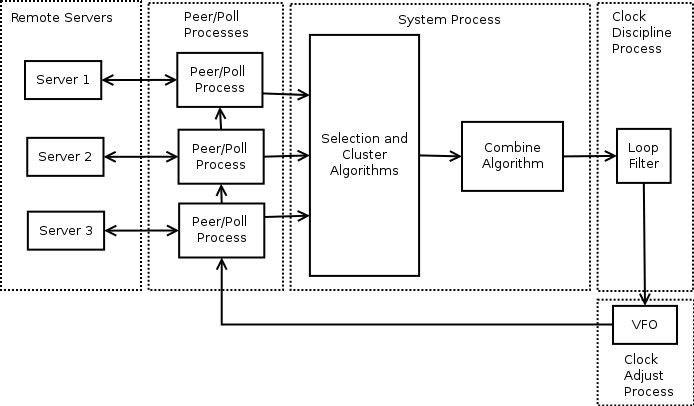
\includegraphics[scale=0.4]{image/ntp_implementation}
    \caption {Implementação dos processos executados por um nó da rede.
    Extraída de \cite{ntpv4rtp}.}
    \label{fig:modelo}
\end{figure} 

\FloatBarrier

Cada componente é, portanto, responsável por uma funcionalidade específica
oferecida pelo NTP. Temos, assim:

\begin {enumerate}[i.]
  \item \textit{Remote servers}: servidores que fornecem sincronização aos nós
  da rede. Tais servidores podem pertencer à mesma rede às quais os clientes
  estão inseridos ou podem ser disponibilizados via Internet por organismos
  responsáveis por gerenciar e garantir que os relógios apresentem tempos
  consistentes. 
  
  A fim de diferenciar os diversos servidores utilizados em relação ao seu grau
  de importância e confiabilidade, o protocolo NTP atribui um nível a cada
  \textit{server}, chamado de \textit{stratum}. Tal atributo vale 1 para
  servidores primários, 2 para servidores secundários e assim sucessivamente. À
  medida que o valor de \textit{stratum} aumenta, a precisão diminui,
  dependendo do estado da rede. O valor máximo deste atributo é 15 e, portanto,
  são permitidos até 15 níveis hierárquicos. O valor 0 é reservado pelo
  protocolo para mensagens de controle e transmissão de estado entre nós. Tais
  mensagens são chamadas de pacotes \textit{Kiss-o'-Death}.
  
%   Caso \textit{stratum} de determinado servidor apresente o valor
%   16, isso significa que o cliente que está tentando obter sincronização está
%   dessincronizado com tal servidor.
  
  \item \textit{Peer/poll processes}: quando um pacote transmitido por um
  servidor chega em um nó, o \textit{peer process} é chamado. Tal processo então
  verifica se o pacote é consistente (\textit{On-Wire protocol}, proteção
  contra perdas e duplicatas) e calcula algumas estatísticas usadas pelos demais
  processos. Tais estatíticas consistem em:
  		
  		\begin{itemize}
  		  \renewcommand\labelitemi{--}
  		  \item \textit{offset} (\(\theta\)): deslocamento de tempo do
  		  relógio do servidor em relação ao relógio do sistema;
  		  \item \textit{delay} (\(\delta\)): tempo que o pacote necessita para
  		  percorrer toda a rede entre cliente e servidor;
  		  \item \textit{dispersion} (\( \epsilon \)): erro máximo inerente à medida
  		  do relógio do sistema;
  		  \item \textit {jitter} (\( \psi \)): raiz do valor quadrático médio dos
  		  \textit{offsets} mais recentes.
  		\end{itemize}
  		
	O \textit{poll process} é responsável, por sua vez, por enviar pacotes aos
	servidores a cada intervalo de \(2^\tau\) segundos. \(\tau\) varia de 3 a 17,
	resultando, assim, em intervalos de 8 segundos a 36 horas. O valor de \(\tau\)
	pode variar durante a execução, sendo modificado pelo algoritmo regulador do
	relógio, que será discutido posteriormente. 
	
	\item \textit{System process}: inclui algoritmos de seleção, clusterização e
	combinação que utilizam as diversas estatísticas obtidas de cada servidor para
	determinar os candidatos mais precisos e confiáveis à sincronização do relógio
	do sistema. As funções de cada algoritmo são, respectivamente:
		
		\begin{itemize}
  		  \renewcommand\labelitemi{--}
  		  \item determinar bons candidatos, isto é, determinar quais servidores
  		  possuem informações de sincronismo efetivamente importantes;
  		  \item determinar os melhores candidatos dentro do conjunto de servidores
  		  julgados importantes no passo anterior;
  		  \item computar estatísticas baseadas nos dados recolhidos dos servidores
  		  presentes no subconjunto escolhido pelo algoritmo de clusterização.
  		\end{itemize}
  	
  	\item \textit{Clock discipline process}: responsável por controlar o tempo e
  	frequência do relógio do sistema;
  	
  	\item \textit{Clock-adjust process}: roda a cada segundo para comunicar aos
  	demais processos os resultados das correções realizadas no relógio do
  	sistema.
  	
\end{enumerate}

% \subsection {Exemplo}
% 
% A rede representada pela figura \ref{fig:redeNTP} foi proposta a fim de testar o
% funcionamento do protocolo NTP. As setas determinam as relações entre os nós e
% as direções representam quais nós fornecem e/ou recebem sincronização. Todos os
% computadores pertencem à mesma rede, isto é, assume-se que há um \textit{router}
% ligando esses nós e responsável pela comunicação com a Internet.
% 
% \FloatBarrier
% 
% \begin{figure}[h]
%     
%     \centering
%     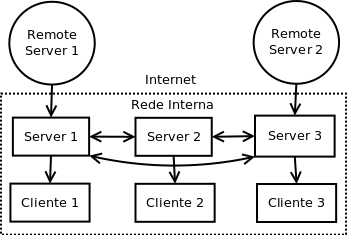
\includegraphics[scale=0.7]{image/rede_ntp_teste}
%     \caption {Topologia da rede de teste.}
%     \label{fig:redeNTP} 
% \end{figure} 
% 
% \FloatBarrier
% 
% Têm-se, portanto, conforme a subseção anterior:
% 
% \begin{itemize}
%   \renewcommand\labelitemi{--}
%   \item associações cliente/servidor entre \textit{remote servers} e
%   \textit{servers}, e entre \textit{servers} e \textit{clients};
%   \item associações simétricas ativas entre \textit{servers}.
% \end{itemize}
% 
% A fim de eliminar a necessidade de implementar essa rede fisicamente,
% utilizou-se o \textit{software virtualbox}. Cada máquina presente na figura, com
% exceção dos \textit{remote servers}, foi substituída por uma máquina virtual,
% cujo sistema operacional é o \textit{Linux Debian 8.2.0 i386}. A escolha deste
% sistema foi baseada nas características previstas para as máquinas que comporão
% a infraestrutura do Sirius. Além disso, como pretende-se isolar completamente a
% rede, isto é, eliminar qualquer comunicação com a Internet, os \textit{remote
% servers} serão substituídos pelos respectivos servidores. Dessa maneira, tais
% servidores utilizarão seus próprios relógios como fonte primária de sincronismo.
% 
% \vspace{12pt}
% 
% Foi adotado que a rede teria endereço \texttt{10.0.0.0/24}, os servidores
% possuiriam endereços do tipo \texttt{10.0.0.10x}, sendo \textit{x} o dígito que
% caracteriza o servidor (1, 2 ou 3), e \texttt{10.0.0.0y1} para os clientes,
% sendo \textit{y} o equivalente de \textit{x}. 
% 
% 
% \vspace{12pt}
% 
% Após a configuração de rede das respectivas máquinas virtuais, a instalação do
% NTP pode prosseguir. Inicialmente, é necessário fazer a instalação do pacote
% \texttt{ntp} através do comando
% 
% \begin{lstlisting}[language=bash, style=nonumbers]
% $ sudo apt-get install ntp
% \end{lstlisting}
% 
% Estão incluídos neste pacote, os programas \texttt{ntpd}, \texttt{ntpq}
% e \texttt{ntpqc}. \texttt{ntpd}, ou \textit{NTP Daemon}, roda continuamente no
% sistema e é responsável pela troca de mensagens com os diversos servidores
% ou clientes, de acordo com as configurações, enquanto que \texttt{ntpq}
% e \texttt{ntpqc} (o \textit{q} refere-se a \textit{query}) são utilizados para
% verificar o estado das variáveis e alterar configurações do \textit{daemon}. 
% 
% \vspace{12pt}
% 
% Quando é iniciado, o \textit{daemon} retira as suas configurações do arquivo
% \texttt{/etc/ntp.conf}. Cada nó da rede deve, portanto,
% configurar esse arquivo de acordo com as funções que desempenha.
% 
% \vspace{12pt}
% 
% A configuração dos clientes é simples: basta adicionarmos a linha
% 
% \begin{lstlisting}[language=bash, style=nonumbers]
% server 10.0.0.10y iburst
% \end{lstlisting}
% 
% ao arquivo de configurações. A opção \texttt{iburst} é uma otimização fornecida
% pelo protocolo que agiliza a sincronização inicial. Essa opção faz com que o
% intervalo de envio de pacotes seja reduzido e a quantidade de pacotes
% enviados seja aumentada caso o servidor não esteja acessível. 
% 
% \vspace{12pt}
% 
% Para o \textit{server 2}, é necessário adicionarmos as duas linhas seguintes.
% 
% \begin{lstlisting}[language=bash, style=nonumbers]
% peer 10.0.0.101
% peer 10.0.0.103
% \end{lstlisting}
% 
% Essas duas linhas criam associações simétricas ativas entre o \textit{server 2}
% e os outros servidores. Dessa maneira, eles poderão trocar informações de
% sincronização entre si.
% 
% \vspace{12pt}
% 
% Para os servidores 1 e 3, além das duas linhas contendo a opção \texttt{peer}, é
% necessário também adicionar as duas linhas abaixo:
% 
% \begin{lstlisting}[language=bash, style=nonumbers]
% server 127.127.0.0
% fudge 127.127.0.0 stratum 1
% \end{lstlisting}
% 
% A primeira opção configura o relógio local do sistema como uma fonte de
% sincronização, enquanto que a segunda aumenta a sua hierarquia. Se o
% atributo \texttt{stratum} vale 1, logo a prioridade do respectivo servidor
% torna-se máxima.
% 
% \vspace{12pt}
% 
% Para iniciar o \textit{daemon}, basta executar o comando abaixo em cada máquina.
% 
% \begin{lstlisting}[language=bash, style=nonumbers]
% $ sudo /etc/init.d/ntp restart
% \end{lstlisting}
% 
% Os sistemas levam alguns minutos para se sincronizarem. Para verificar o estado
% das conexões e da sincronização, utiliza-se o programa \texttt{ntpq} através do
% comando 
% 
% \begin{lstlisting}[language=bash, style=nonumbers]
% $ ntpq -p
% \end{lstlisting}
% 
% A opção \texttt{-p} lista todos os nós utilizados para sincronização do relógio
% local. Para o \textit{Server 1}, espera-se uma saída parecida com a figura
% \ref{fig:sv1} (não há garantias que seja idêntica, visto que os algoritmos que
% determinam as fontes que serão utilizadas para sincronização são baseados em
% fatores que podem variar dependendo do estado da rede). 
% 
% \FloatBarrier
% 
% \begin{figure}[h]
%     
%     \centering
%     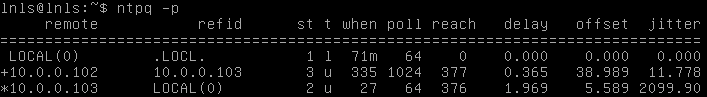
\includegraphics[scale=0.7]{image/server1_screen}
%     \caption {Resultado do comando \texttt{ntpq -p} no \textit{Server 1}.}
%     \label{fig:sv1} 
% \end{figure} 
% 
% \FloatBarrier
% 
% O caracter \texttt{*} indica quais dos servidores está sendo usado como fonte de
% sincronismo e o \texttt{+} indica os outros possíveis candidatos válidos (os
% chamados \textit {truechimers}). É possível também encontrar o caracter
% \texttt{-}, representando servidores que provêm fontes de sincronismo inválidas
% (chamadas também de \textit{falsetickers}). \texttt{refid} representa o
% \textit{id} da refêrencia de sincronismo do respectivo servidor. Por exemplo, o
% nó \texttt{10.0.0.103} usa como referência o relógio \texttt{LOCAL(0)}, que o
% próprio relógio da máquina. \texttt{st} é o valor do \textit{stratum}. Conforme
% esperado, servidores secundários, como \texttt{10.0.0.103}, que possuem somente
% uma fonte de sincronismo, têm esse atributo setado para 2. \texttt{when}
% corresponde ao tempo, em segundos, da última troca de pacotes e \texttt{poll} é
% o tempo em segundos até o próximo envio. \texttt{reach}, em representação octal,
% indica se as 8 últimas tentativas de comunicação foram bem-sucedidas ou não. 
% Esse atributo funciona como um registrador que é deslocado para a esquerda a
% cada nova comunicação. Se ela for bem-sucedida, o \textit {bit} mesmo
% significativo é setado para 1, senão, para 0. As demais colunas são as
% estatísticas comentadas na subseção anterior.
% 
% \vspace{12pt}
% 
% A figura \ref{fig:cl1} é a saída do comando \texttt{ntpq -p} no cliente
% conectado no \textit{server 1}. Conforme esperado, ele obtem corretamente a
% sincronização deste servidor.
% 
% \FloatBarrier
% 
% \begin{figure}[h]
%     
%     \centering
%     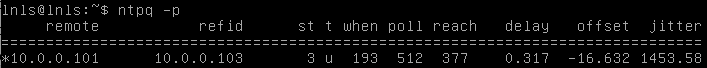
\includegraphics[scale=0.7]{image/client1_screen}
%     \caption {Resultado do comando \texttt{ntpq -p} no \textit{Client 1}.}
%     \label{fig:cl1}  
% \end{figure} 

\FloatBarrier
\subsection {Aplicação ao sistema de controle do \textit{Sirius}}

Considerando que o sistema de controle do \textit{Sirius} será composto por uma
vasta quantidade de \textit{Beagles} e \textit{hosts} conectados, é de extrema
importância que a data e hora de todas elas estejam corretamente sincronizadas
entre si, a fim de garantir a coerência entre os diversos \textit{logs} e
\textit{timestamps} de variáveis EPICS que serão gerados na execução dos
programas. Conforme discutido na subseção anterior, um servidor NTP é capaz de
fornecer sincronismo a um número variável de clientes, desde que eles estejam
configurados a obter sincronização deste servidor.

\vspace{12pt}  

Diversos institutos fornecem, através da Internet, relógios de referência, isto
é, servidores chamados de \textit{stratum 1}, obtidos a partir de equipamentos
como \textit{GPS}, relógios atômicos ou outros \textit{radio clocks}. Para a rede
de controle do \textit{Sirius}, que pretende ser totalmente isolada de redes
externas, tal solução não pode ser obviamente utilizada. Sendo assim, propõe-se
a implementação de um servidor NTP \textit{stratum 1} a partir de um GPS
\textit{receiver}, ligado a uma \textit{BeagleBone Black} dedicada, que
hospedará o servidor.

\vspace{12pt}

\textit{GPS receivers} são capazes de fornecer, além do posicionamento e
velocidade, data e hora no padrão \textit{UTC} e um pulso, chamado de
\textit{1PPS}, com frequência de 1Hz e precisão na ordem de 50ns
\cite{gpsdhowto}. Pode-se imaginar que somente o horário fornecido é suficiente
para a implementação de um bom servidor NTP. Entretanto, os \textit{delays} com
que tal informação é recebida e transmitida pelo \textit{receiver} não são
constantes e variam conforme alguns parâmetros como temperatura e qualidade do
sinal \cite{rasp}. Dessa forma, a fim de obter um tempo preciso, é necessário o
uso do pulso de 1PPS, cuja finalidade é marcar o ínicio de um novo segundo. A combinação
destes dois últimos, aliados a um sistema operacional com \textit{kernel}
habilitado ao tratamento de tais pulsos, permite a implementação de um servidor
com acurácia da ordem de microssegundos em relação ao horário \textit{real}. É
importante destacar que o PPS deve ser combinado com alguma outra fonte de
tempo, uma vez que ele não capaz de dizer o horário efetivo, isto é, horas,
minutos e segundos, mas somente o início de um novo segundo.

\vspace{12pt}

As próximas subseções descrevem o \textit{hardware} utilizado e a
configuração do servidor NTP.

\subsubsection{Descrição do \textit{hardware}}

No total, utilizou-se três modelos diferentes de receptores GPS, sendo que dois
deles tratam-se de \textit{kits} contendo módulos GPS já integrados. Escolhemos,
em um primeiro momento, os \textit{kits} \textit{Ultimate GPS Breakout} da
\textit{Adafruit} e \textit{GPS Click} da \textit{MikroElektronika}. O terceiro
modelo, por sua vez, é o módulo receptor \textit{CAM M8Q} da \textit{ublox}, que
foi posteriormente incluído em uma placa desenvolvida e fabricada durante o
estágio. As principais vantagens do modelo \textit{CAM-M8Q} são o menor custo
(\$25 contra \$39.95 e \$49 dos dois \textit{kits}, respectivamente) e maior
independência no projeto do circuito de integração.

\vspace{12pt}

Todos fornecem um pino de saída 1PPS e comunicação serial assíncrona
\textit{RX/TX} (\textit{UART}). Foi utilizado também o multivibrador mono
estável \textit{74HC123}, a fim de obtermos um pulso 1PPS mais largo na entrada
do pino da \textit{BeagleBone Black}. Tal pulso é fornecido por receptores mais
antigos com uma largura de apenas \(10\mu s\), que pode não ser capturado pelo
\textit{kernel} do sistema operacional da placa, dependendo, evidentemente, da
utilização da sua CPU. Sendo assim, utilizando-se um resistor de \(1M\Omega\) e
um capacitor de \(1\mu F\) conectados ao \textit{74HC123}, obtém-se uma largura
de aproximadamente \(500 ms\) na saída deste \textit{chip}. Para os receptores
listados acima, porém, o uso do multivibrador não é necessário, visto que todos provêem pulsos de largura superiores a 100\(ms\).

\subsubsection{Configuração do servidor NTP}

O primeiro passo para a configuração foi verificar se o \textit{kernel} do
\textit{Linux} está provido do módulo \textit{LinuxPPS}, responsável pela
captura de pulsos 1PPS. Versões superiores à 2.6.34 já integram tal módulo por
padrão \cite{linuxpps}. A segunda etapa consistiu na configuração das portas de
entrada e saída que serão usadas pela \textit{BeagleBone Black} para se comunicar com o
GPS. Ela foi realizada a partir da implementação de um arquivo de extensão
\textit{DTS}, cujo objetivo é modificar a função interna dos pinos da
\textit{Beagle}. 3 pinos, portanto, foram utilizados: 2 para o par
\textit{RX/TX} e um para a entrada PPS. 

\vspace{12pt}

Em seguida, configurou-se os \textit{daemons} \textit{GPSD}, que implementa o
protocolo de comunicação NMEA e realiza a troca de informação com o receptor
GPS, e \textit{NTPD}, responsável por ajustar o tempo do sistema, conforme
seções anteriores. A comunicação entre estes dois processos é realizada por meio de um
espaço de memória compartilhado disponível. É necessário certificar-se, ainda,
que o \textit{NTPD} foi compilado com o \textit{driver ATOM}, que se encarrega
do processamento dos pulsos PPS.

% A segunda etapa consiste na configuração das portas de entrada e
% saída que serão usadas pela \textit{BeagleBone Black} para se comunicar com o
% GPS. Conforme referência [1], adotaremos que os pinos \texttt{P9-11} e
% \texttt{P9-13} serão utilizados, respectivamente, como \textit{TX} e
% \textit{RX}, e \texttt{P9-12}, como entrada do pulso 1PPS. O arquivo de
% \textit{device tree overlay} especificando tais comportamentos pode ser obtido
% a partir de \url{http://tinyurl.com/oeo2ccu}. Após compilado e carregado, duas
% novas  interfaces estarão disponíveis, sendo elas \path{/dev/ttyO4} e
% \path{/dev/pps0}. Para habilitar o carregamento deste \textit{overlay} após o
% \textit{boot}, é necessário editar os arquivos \path{/boot/uEnv.txt} e
% \path{/etc/default/capemgr} com, respectivamente,
% \path{cape_enable=capemgr.enable_portno=overlay_GPS} e \path{CAPE=overlay_GPS}.
% 
% \vspace{12pt}
%  
% A comunicação com o \textit{GPS receiver} é realizado por meio do
% \textit{daemon GPSD}. Após instalá-lo, crie o arquivo
% \path{/lib/systemd/system/gpsd.service} e adicione as seguintes linhas:
% 
% \begin{lstlisting}[keywordstyle=\ttfamily, style=nonumbers]
% [Unit]
% Description=GPS (Global Positioning System) Daemon
% Requires=gpsd.socket
% 
% [Service]
% ExecStart=/usr/sbin/gpsd -n -N /dev/ttyO4
% 
% [Install]
% Also=gpsd.socket
% \end{lstlisting}
% 
% O \textit{daemon} pode ser iniciado com
%  
% \begin{lstlisting}[keywordstyle=\ttfamily, style=nonumbers]
% systemctl start gpsd.service
% \end{lstlisting}
% 
% O programa \texttt{gpsmon}, provido no pacote
% \path{gpsd-clients}, permite verificar se a conexão entre a \textit{BeagleBone}
% o módulo GPS está correta.
% 
% \vspace{12pt}
% 
% A configuração do NTP é ligeiramente mais complicada, visto que é necessário
% recompilá-lo de maneira a habilitar o uso do \textit{driver} responsável por
% manipular o pulso 1PPS. Para tal, faça o \textit{download} do código fonte em
% \url{http://www.ntp.org/downloads.html} e extraia seu conteúdo para o diretório
% de preferência. Em seguida, entre neste diretório e execute o comando abaixo. As
% \textit{flags} \texttt{--enable-ATOM} e \texttt{--prefix} especificam,
% respectivamente, a ativação do \textit{driver} de gerenciamento do 1PPS e o
% diretório onde o NTP será instalado.
% 
% \begin{lstlisting}[keywordstyle=\ttfamily, style=nonumbers]
% ./configure --enable-ATOM --prefix=/usr/local/ --enable-linuxcaps
% \end{lstlisting}
% 
% \vspace{12pt}
% 
% O comando \texttt{make install} instalará os binários no diretório especificado.
% O pacote \texttt{libcap-dev} é necessário e, portanto, deve ser instalado via
% \texttt{apt-get install}. Enfim, a última etapa consiste em atualizar os
% arquivos \texttt{ntpdate.service} e \texttt{ntpd.service} para que os serviços sejam
% inicializados assim que a \textit{BeagleBone} for ligada. Para tal, implementei
% um \textit{script bash}, encontrado no repositório do grupo, que
% realiza automaticamente esta tarefa.

\subsubsection{Implementação de variáveis EPICS}
\label{sec:pvsgps}

Duas implementações de servidores de variáveis EPICS foram escritas. A primeira,
desenvolvida em \textit{Python}, extende as classes presentes no módulo
\textit{PCASpy} e utiliza os módulos \texttt{python-gps} e \texttt{ntplib} para
comunicar-se com os \textit{daemons} \textit{GPSD} e \textit{NTPD},
respectivamente. A segunda, por sua vez, consiste em uma ponte, escrita em C,
entre o \textit{Stream IOC}, que se trata de uma aplicação desenvolvida pelo
Grupo baseada no \textit{StreamDevice}, e as bibliotecas \texttt{libntpq} e
\texttt{libgps}.
De modo geral, o \textit{Stream IOC} envia requisições, seguindo o protocolo
BSMP, via um \textit{socket unix} local para a \textit{ponte}, que utiliza, por
sua vez, as bibliotecas \texttt{libntpq} e \texttt{libgps} para obter os valores. Vale
destacar que a \texttt{libntpq} não está disponível nos repositórios oficiais da
maioria dos sistemas Linux atuais e, portanto, deve ser compilada separadamente
a partir do código fonte do \textit{NTPD}.

\vspace{12pt}

As variáveis EPICS servidas pelas implementações foram divididas em duas
categorias principais, de acordo com a sua origem, isto é, se elas
descrevem parâmetros do servidor NTP ou dados recebidos do receptor GPS. A
tabela \ref{tab:ntpd} resume as principais variáveis geradas pelo servidor e a
\ref{tab:gpsd}, para o módulo GPS. A interface representada na figura
\ref{img:ntp-opi}, construída no \textit{OPI Builder} do \textit{Control System
Studio}, foi gerada a partir destas bibliotecas e referencia as \textit{PVs}
descritas nas tabelas a seguir. A figura ilustra o início do processo de
sincronização do \textit{clock} do \textit{host}. Desse modo, verifica-se um
grande \textit{offset} inicial e uma diminuição gradativa desta medida.

\begin{table}[h]

	\centering
	\caption{\label{tab:ntpd} Variáveis definidas para o servidor
	\textit{NTPD}.}
	\begin{tabular}{| c | p{.70\textwidth} |}
		\hline
		\textbf{Nome} & \textbf{Descrição} \\	\hhline{|=|=|}
		\texttt{NTP:Leap} & Indicação de um eventual \textit{leap second} pendente a
		ser inserido ou removido. \\
		\hline \texttt{NTP:Stratum} & \textit{Stratum} do servidor \\ \hline
		\texttt{NTP:Refid} & ID de referência da fonte de sincronismo \\ \hline
		\texttt{NTP:Offset} & \textit{Offset} de tempo entre o relógio do sistema e da
		fonte de sincronismo \\
		\hline \texttt{NTP:Jitter} & Desvio padrão das medidas de \textit{offset} mais
		recentes \\ \hline 
		\texttt{NTP:Precision} & Precisão do \textit{clock} do sistema em
		\textit{log2} \\
		\hline \texttt{NTP:Srcadr} & Endereço IP do servidor \\ \hline 			
		\texttt{NTP:Version} & Versão do \textit{daemon} NTPD e data de compilação \\
		\hline \texttt{NTP:Timestamp} & Diferença, em segundos, entre a data atual do
		servidor e a \textit{unix epoch} (1 de Janeiro de 1970). \\ \hline
	\end{tabular}	    
\end{table}

\begin{table}[h]
	\centering
	\caption{\label{tab:gpsd} Variáveis definidas para o receptor
	\textit{GPS}.}
	\begin{tabular}{| c | l |}
		\hline
		\textbf{Nome} & \textbf{Descrição} \\	\hhline{|=|=|}
		\texttt{GPS:Fix} & Indicação do tipo de \textit{fix} (\textit{No fix},
		2D ou 3D \textit{fix})	\\ \hline  
		\texttt{GPS:Latitude} & Latitude medida pelo GPS \\ \hline
		\texttt{GPS:Longitude} & Longitude medida pelo GPS \\ \hline
		\texttt{GPS:Altitude} & Altitude medida pelo GPS \\ \hline
		\texttt{GPS:Sattelites} & \textit{String} contendo a identificação dos
		satélites usados para o \textit{fix} \\ \hline 
		\texttt{GPS:Timestamp} & \textit{Timestamp} fornecido, análogo à mesma
		variável do servidor NTP. \\ \hline
	\end{tabular}	   

\end{table}

% \begin{itemize}
%   \renewcommand\labelitemi{--}
%   \item \textit{\texttt{NTP:OnOff}}: indica se o servidor está ativo.
%   
%   \item \textit{\texttt{NTP:Address}}: endereço IP do servidor na rede.
%   
%   \item \textit{\texttt{NTP:Timestamp}}: número de segundos entre a data do
%   servidor e 01 Janeiro de 1970.
%   
%   \item \textit{\texttt{NTP:Day}}, \textit{\texttt{NTP:Month}},
%   \textit{\texttt{NTP:Year}}, \textit{\texttt{NTP:Hour}},
%   \textit{\texttt{NTP:Minute}} e \textit{\texttt{NTP:Second}}:
%   conversão de \textit{\texttt{NTP:Timestamp}} nos respectivos campos.
%   
%   \item \textit{\texttt{NTP:Stratum}}: \textit{stratum} do servidor.
%   
%   \item \textit{\texttt{NTP:Leap}}: ocasionalmente, as autoridades adicionam
%   ou retiram 1 segundo do horário UTC, com o intuito de torná-lo mais
%   próximo do horário solar. Esta variável pode assumir 4 estados, de acordo
%   com a RFC5905. Quando vale 0, significa que nenhuma mudança é necessária e
%   quando vale 1 ou 2, um segundo é, respectivamente, adicionado ou retirado. Ela
%   pode conter também o valor 3, que representa que o relógio do servidor está
%   dessincronizado.
% 
%   \item  \textit{\texttt{NTP:Version}}: versão no NTP. Por padrão, sempre
%   utilizamos a 4.
% 
%   \item  \textit{\texttt{NTP:Roundtrip}}: tempo que o pacote de requisição leva
%   para chegar e retornar da fonte, em milissegundos.
% 
%   \item \textit{\texttt{NTP:Reference}}: \textit{string} de 4 caracteres que
%   identifica a fonte de sincronismo atualmente utilizado pelo servidor.
% \end{itemize}
% 
% Para os receptores GPS, por sua vez, são disponibilizadas:
% 
% \begin{itemize}
% 
%   \renewcommand\labelitemi{--}
%   \item \textit{\texttt{GPS:Fix}}: \textit{enum} que indica o tipo de
%   \textit{fix} obtido pelo GPS. 0 indica que o receptor não pôde obter nenhum
%   \textit{fix}, 1 que um \textit{2D fix} foi obtido e 2, um \textit{3D fix}.
%   
%   \item \textit{\texttt{GPS:Latitude}}, \textit{\texttt{GPS:Longitude}} e
%   \textit{\texttt{GPS:Altitude}}:  informações de posicionamento.
% 
%   \item \textit{\texttt{GPS:UTC:Timestamp}}: horário UTC em
%   formato \textit{timestamp} retornado pelo GPS. Da mesma maneira, são
%   disponibilizadas variáveis individuais contendo campos, tais como dia, mês e
%   ano, obtidos a partir deste \textit{timestamp}.
%   
%   \item  \textit{\texttt{GPS:UTC:Satellites}}: vetor com os \textit{PRN} dos
%   satélites utilizados no cálculo do \textit{fix}.
% \end{itemize}
% 

\begin{figure}[h]
    
    \centering
    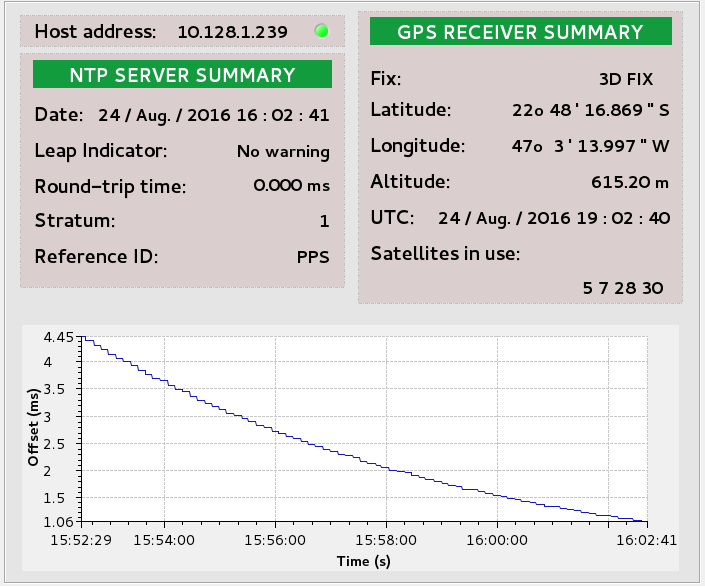
\includegraphics[scale=0.35]{image/epics-opi-ntpgps}
    \caption {Interface construída para visualização das
    \textit{PVs}.}
    \label{img:ntp-opi} 
\end{figure} 

 
\subsection{Projeto de \textit{capes} para a \textit{BeagleBone Black}}

Três \textit{capes} foram construídos através do \textit{Kicad}, um para cada
receptor GPS, e fabricados na prototipadora \textit{LPKF}. Os \textit{layouts
PCB} podem ser encontrados no repositório \textit{GIT} do grupo.

\subsection{Resultados}

A figura \ref{img:adafruit} apresenta os resultados obtidos para o receptor
\textit{Adafruit Ultimate GPS Breakout}. Tal tabela foi obtida através do
comando \texttt{ntpq}, sendo que as colunas representam informações relativas às fontes de sincronismo que
tal servidor utiliza, tais como \textit{stratum}, \textit{delay},
\textit{offset} e \textit{jitter}, cujos conceitos já foram explorados
anteriormente. Destaca-se a presença de duas fontes específicas, \texttt{SHM} e
\texttt{PPS}. A primeira, cuja representação é a abreviação de \textit{SHared
Memory}, obtém seus valores de hora e data por meio de um segmento compartilhado de memória,
acessado igualmente pelo utilitário \texttt{gpsd}. A segunda trata-se da fonte
ligada ao PPS, controlada pelo \textit{driver} \texttt{ATOM} que tivemos que
incorporar na compilação do \textit{NTP} e que utiliza a API \textit{timepps}
para se comunicar com o \textit{kernel}. A fonte representada por
\texttt{LOCAL}, que obtém a data do próprio sistema, é considerada apenas se as duas anteriores
não estiverem disponíveis.

\begin{figure}[h]
    
    \centering
    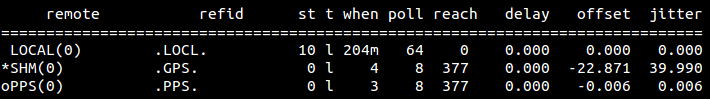
\includegraphics[scale=0.6]{image/adafruit_GPS}
    \caption {Comando \texttt{ntpq -p} na
    \textit{BeagleBone} conectada ao \textit{cape} com o receptor
    \textit{Adafruit Ultimate GPS}.}
    \label{img:adafruit} 
\end{figure} 

\vspace{12pt}

Conforme esperado, o servidor conseguiu sincronizar-se ao início de um novo
segundo (PPS) com precisão e \textit{offset} na ordem de unidades de
microssegundos. Na tabela representada acima, por exemplo, o \textit{offset} é
-0.006ms, isto é, o horário do servidor está 6\(\mu s\) atrás do pulso de
PPS, e o jitter, 0.006 ms.

\vspace{12pt}

A figura \ref{img:mikroe}, por sua vez, exibe o resultado da execução do mesmo
comando, porém para o receptor \textit{MikroE GPS Click}. Observa-se que,
como no caso anterior, o servidor conseguiu sincronizar-se ao pulso de PPS.
Enfim, a figura \ref{img:cliente_ntp} representa a saída do comando executado em
uma \textit{Beagle} que utiliza 3 servidores para obter o horário. Os dois
primeiros (\texttt{10.0.6.63} e \texttt{10.0.6.60}) são os endereços das placas
ligadas, respectivamente, aos receptores da \textit{Adafruit} e da
\textit{MikroE}, e o último, enfim, é um servidor externo, referenciado pelo
endereço \url{ntp.cnpem.br}.  Nota-se que a diferença entre as fontes PPS está
na ordem de unidades de microssegundos e que a diferença entre elas e a externa
é da ordem de 100\(\mu s\). Os testes para o módulo da \textit{ublox} não foram
concluídos antes da redação deste relatório, portanto não estão incluídos.

\begin{figure}[h]
    \centering
    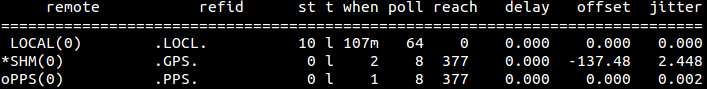
\includegraphics[scale=0.6]{image/mikroe}
    \caption {Comando \texttt{ntpq -p} na
    \textit{BeagleBone} conectada ao \textit{cape} com o receptor \textit{MikroE
    GPS Click}.}  
    \label{img:mikroe} 
\end{figure} 

\begin{figure}[h!]
    
    \centering
    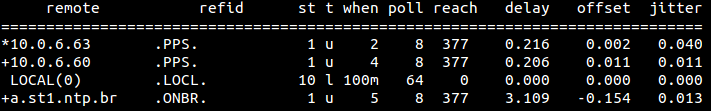
\includegraphics[scale=0.6]{image/cliente-ntp}
    \caption {Comando \texttt{ntpq -p} na \textit{BeagleBone} cliente que obtêm sincronização de 3 servidores distintos.}
    \label{img:cliente_ntp} 
\end{figure} 